\par\vspace{1em}
\begin{longtable}{|c|c|c|}
  \hline
  \rule[-0.5em]{0pt}{1.8em} & \rule[-0.5em]{0pt}{1.8em} $G$ & \rule[-0.5em]{0pt}{1.8em} $M$ \\
  \hline
  \endhead
  \hline
  \endfoot
  \caption{Grafos y sus matrices de adyacencia} \label{tab:grafos_matrices} \\
  \endlastfoot

  $G_1 - M_1$ &
  \begin{minipage}{0.3\textwidth} \centering \vspace{8pt} \resizebox{0.85\linewidth}{!}{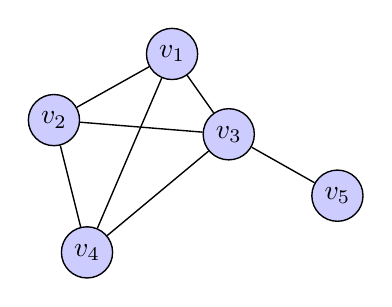
\begin{tikzpicture}[
  scale=0.6,
  vnode/.style={circle, fill=blue!20, draw=black, line width=0.5pt, inner sep=2pt, minimum size=6.5mm},
  edge/.style={line width=0.5pt, draw=black}
]

  % Posicionamiento de vértices asimétrico
  \node[vnode] (v1) at (0, 3.2) {$v_1$};
  \node[vnode] (v2) at (-2.5, 1.8) {$v_2$};
  \node[vnode] (v3) at (1.2, 1.5) {$v_3$};
  \node[vnode] (v4) at (-1.8, -1.0) {$v_4$};
  \node[vnode] (v5) at (3.5, 0.2) {$v_5$};

  % Aristas
  \draw[edge] (v1) -- (v2);
  \draw[edge] (v1) -- (v3);
  \draw[edge] (v2) -- (v4);
  \draw[edge] (v3) -- (v4);
  \draw[edge] (v3) -- (v5);
  \draw[edge] (v2) -- (v3);
  \draw[edge] (v1) -- (v4);

\end{tikzpicture}
} \vspace{6pt} \end{minipage} &
  \begin{minipage}{0.3\textwidth} \centering \vspace{8pt}
    $\begin{pmatrix}
      0 & 1 & 1 & 1 & 0 \\
      1 & 0 & 1 & 1 & 0 \\
      1 & 1 & 0 & 1 & 1 \\
      1 & 1 & 1 & 0 & 0 \\
      0 & 0 & 1 & 0 & 0
    \end{pmatrix}$
  \vspace{6pt} \end{minipage} \\
  \hline

  $G_2 - M_2$ &
  \begin{minipage}{0.3\textwidth} \centering \vspace{8pt} \resizebox{0.85\linewidth}{!}{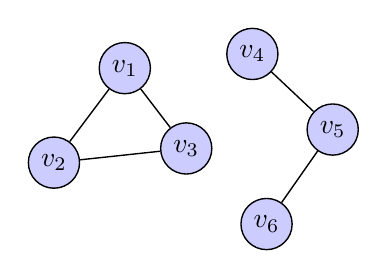
\begin{tikzpicture}[
  scale=0.6,
  vnode/.style={circle, fill=blue!20, draw=black, line width=0.5pt, inner sep=2pt, minimum size=6.5mm},
  edge/.style={line width=0.5pt, draw=black}
]

  % --- Componente 1 (Triángulo) ---
  \node[vnode] (v1) at (-2.5, 2.5) {$v_1$};
  \node[vnode] (v2) at (-4.0, 0.5) {$v_2$};
  \node[vnode] (v3) at (-1.2, 0.8) {$v_3$};

  \draw[edge] (v1) -- (v2) -- (v3) -- (v1);

  % --- Componente 2 (Camino/Trayectoria) ---
  \node[vnode] (v4) at (0.2, 2.8) {$v_4$};
  \node[vnode] (v5) at (1.9, 1.2) {$v_5$};
  \node[vnode] (v6) at (0.5, -0.8) {$v_6$};

  \draw[edge] (v4) -- (v5);
  \draw[edge] (v5) -- (v6);

\end{tikzpicture}
} \vspace{6pt} \end{minipage} &
  \begin{minipage}{0.3\textwidth} \centering \vspace{8pt}
    $\begin{pmatrix}
      0 & 1 & 1 & 0 & 0 & 0 \\
      1 & 0 & 1 & 0 & 0 & 0 \\
      1 & 1 & 0 & 0 & 0 & 0 \\
      0 & 0 & 0 & 0 & 1 & 0 \\
      0 & 0 & 0 & 1 & 0 & 1 \\
      0 & 0 & 0 & 0 & 1 & 0
    \end{pmatrix}$
  \vspace{6pt} \end{minipage} \\
  \hline

  $G_3 - M_3$ &
  \begin{minipage}{0.3\textwidth} \centering \vspace{8pt} \resizebox{0.85\linewidth}{!}{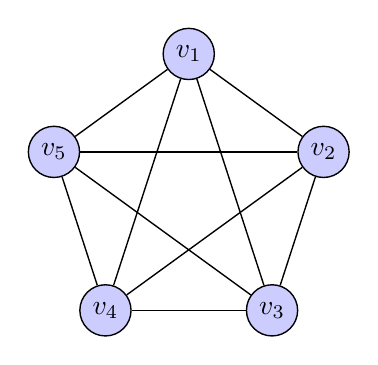
\begin{tikzpicture}[
  scale=1.0,
  vnode/.style={circle, fill=blue!20, draw=black, line width=0.5pt, inner sep=2pt, minimum size=6.5mm},
  edge/.style={line width=0.5pt, draw=black}
]

  % Vértices dispuestos en pentágono regular para máxima simetría
  \node[vnode] (v1) at (90:1.8) {$v_1$};
  \node[vnode] (v2) at (162:1.8) {$v_5$};
  \node[vnode] (v3) at (234:1.8) {$v_4$};
  \node[vnode] (v4) at (306:1.8) {$v_3$};
  \node[vnode] (v5) at (18:1.8) {$v_2$};

  % Todas las conexiones de un grafo completo K5 (10 aristas)
  \draw[edge] (v1) -- (v2);
  \draw[edge] (v1) -- (v3);
  \draw[edge] (v1) -- (v4);
  \draw[edge] (v1) -- (v5);

  \draw[edge] (v2) -- (v3);
  \draw[edge] (v2) -- (v4);
  \draw[edge] (v2) -- (v5);

  \draw[edge] (v3) -- (v4);
  \draw[edge] (v3) -- (v5);

  \draw[edge] (v4) -- (v5);

\end{tikzpicture}
} \vspace{6pt} \end{minipage} &
  \begin{minipage}{0.3\textwidth} \centering \vspace{8pt}
    $\begin{pmatrix}
      0 & 1 & 1 & 1 & 1 \\
      1 & 0 & 1 & 1 & 1 \\
      1 & 1 & 0 & 1 & 1 \\
      1 & 1 & 1 & 0 & 1 \\
      1 & 1 & 1 & 1 & 0
    \end{pmatrix}$
  \vspace{6pt} \end{minipage} \\
  \hline
\end{longtable}
\par\vspace{-0.3em}
